\documentclass[12pt]{article}

%Russian-specific packages
%--------------------------------------
\usepackage[T2A]{fontenc}
\usepackage[utf8]{inputenc}
\usepackage[english, russian]{babel}
%--------------------------------------
%for search in russian
\usepackage{cmap}

%Math-specific packages
%--------------------------------------
\usepackage{amsmath}
\usepackage{amssymb}

%Format-specific packages
%--------------------------------------
\usepackage[left=2cm,
            right=2cm,
            top=2cm,
            bottom=2cm,
            bindingoffset=0cm]{geometry}
%--------------------------------------

\usepackage{amsthm}

\newtheorem*{definition}{Определение}
\newtheorem*{theorem}{Теорема}

%Roman enum items
\usepackage{enumerate}

\def\bigO{ \underline{\underline{\mathcal{O}}} }

%Manage images
\usepackage{graphicx}
\graphicspath{ {data/} }

\begin{document}
\begin{center}
	Численное решение дифференциального уравнения второго порядка. Отчет.
\end{center}
\begin{center}
	Шерстобитов Андрей, задача 4
\end{center}
Общая постановка задачи:
\[\begin{cases}
		-y''(x) +p(x)y(x) = f(x),\ p(x) \geq 0 \\
		y(0) = 0                               \\
		y'(1) = 0
	\end{cases}\]
Предлагается исследовать разностную схему вида
\[\begin{cases}
		-\frac{y_{k+1}-2y_k+y_{k-1}}{h^2}+p_ky_k = f_k,\ h = \frac{2}{2N-1},\ 1 \leq k \leq N-1 \\
		x_k = kh,\ f_k := f(x_k),\ p_k := p(x_k)                                                \\
		y_0 = 0                                                                                 \\
		y_N = y_{N-1}
	\end{cases}\]
Запишем канонический вид. Найдем коэффициенты для краевых условий
\begin{align*}
	k & = 1: \frac{y_2 - 2y_1}{h^2} + p_1y_1= f_1                         \\
	k & = N-1: \frac{-y_{N-1} + y_{N-2}}{h^2} + p_{N-1} y_{N-1} = f_{N-1}
\end{align*}
Задача в матричном виде имеет вид:
\[
	-\left(\begin{array}{cccccc}
			\frac{-2}{h^2} & \frac{1}{h^2}  &               &               &                & 0              \\
			\frac{1}{h^2}  & \frac{-2}{h^2} & \frac{1}{h^2} &               &                &                \\
			               &                & \cdots        & \cdots        &                &                \\
			               &                &               & \frac{1}{h^2} & \frac{-2}{h^2} & \frac{1}{h^2}  \\
			0              &                &               &               & \frac{1}{h^2}  & \frac{-1}{h^2} \\
		\end{array}\right)
	\left(\begin{array}{c}
			y_{1}   \\
			\\
			\vdots  \\
			\\
			y_{N-1} \\
		\end{array}\right)
	+
	\left(\begin{array}{ccc}
			p_1 &        & 0       \\
			    &        &         \\
			    & \ddots &         \\
			    &        &         \\
			0   &        & p_{N-1} \\
		\end{array}\right)
	\left(\begin{array}{c}
			y_{1}   \\
			\\
			\vdots  \\
			\\
			y_{N-1} \\
		\end{array}\right)
	=
	\left(\begin{array}{c}
			f_{1}   \\
			\\
			\vdots  \\
			\\
			f_{N-1} \\
		\end{array}\right)
\]
Будем использовать сеточную интегральную норму
\[\Vert y_h\Vert^2_h = (y_h,y_h)_h= \sum_{k=1}^{N-1}y^2_kh\]
согласованной с нормой $\Vert y(x)\Vert^2_{L^2(0,1)} = \int_0^1y^2(x)dx$ исходной задачи.

План:
\begin{enumerate}[I.]
	\item Доказать, что разностная схема имеет порядок аппроксимации $O(h^2)$.
	\item Доказать устойчивость разностный схемы.
	\item Доказать, что есть сходимость $O(h^2)$.
	\item Выписать алгоритм решения для метода Фурье и метода прогонки.
	\item Показать, что сходимость численно действительно $O(h^2)$ либо иначе.
\end{enumerate}

\newpage

\begin{enumerate}[I.]
	\item Докажем аппроксимацию второго порядка на решении:
	      \begin{enumerate}
		      \item $\Vert L_h(y)_{Y_h}-f_h\Vert_{F_h}\leq\bigO(h^2)$
		            \[\max_{x_k}\left|-\frac{y(x_k+h)-2y(x_k)+y(x_k-h)}{h^2}+p(x_k)y(x_k)-f(x_k)\right|=\]
		            \[y(x_k\pm h)=y(x_k)\pm hy'(x_k)+\frac{h^2}{2}y''(x_k)\pm\frac{h^3}{6}y'''(x_k)+\bigO(h^4)\]
		            \[=\max_{x_k}\left|-\frac{h^2y''(x_k)+\bigO(h^4)}{h^2}+p(x_k)y(x_k)-f(x_k)\right|=\]
		            \[=\max_{x_k}\left|-y''(x_k)+\bigO(h^2)+p(x_k)y(x_k)-f(x_k)\right|=\bigO(h^2)\]
		      \item $\Vert l_h(y)_{Y_h}-\varphi_h\Vert_{\Phi_h}\leq\bigO(h^2)$
		            \[y_0 = 0:\ \Vert y(0)-0\Vert_{\Phi_h}=0\]
		            \begin{multline*}
			            \frac{y_N - y_{N-1}}{h} = 0:\ \left\Vert\frac{y\left(1+\frac{h}{2}\right)-y\left(1-\frac{h}{2}\right)}{h}\right\Vert_{\Phi_h}= \\
			            y\left(1\pm \frac{h}{2}\right)=y(1)\pm \frac{h}{2}y'(1)+\frac{h^2}{2}y''(x_k)+\bigO(h^3) \\
			            =\left\Vert y'(1)+\bigO(h^2)\right\Vert_{\Phi_h}=\bigO(h^2)
		            \end{multline*}
		      \item Условия нормировки
		            \begin{align*}
			            \lim_{h\rightarrow0}\Vert f_h-(f)_{F_h}\Vert_{F_h}                   & =0 \Rightarrow f(x_k)-f(x_k) = 0       \\
			            \lim_{h\rightarrow0}\Vert \varphi_h-(\varphi)_{\Phi_h}\Vert_{\Phi_h} & =0 \Rightarrow (0\ 0)^T - (0\ 0)^T = 0
		            \end{align*}
	      \end{enumerate}
	      Значит схема имеет \textbf{второй порядок аппроксимации}.

	      \textbf{Замечание}: Доказали аппроксимацию на решении в $\Vert\cdot\Vert_e$, но
	      \[\sqrt{\left(\sum_{i=1}^{N-1}x_i^2h\right)}\leq\max|x_i|\sqrt{\left(\sum_{i=1}^{N-1}h\right)}=\max|x_i|\leq C h^2\]
	      То есть из аппроксимации в $\Vert\cdot\Vert_e$ следует аппроксимация в $\Vert\cdot\Vert_h$.

	      \newpage

	\item Напомним определение устойчивости разностной схемы.
	      \begin{definition}
		      Пусть уравнение $y''(x)=f(x)$ доопределено краевыми
		      условиями на разных концах отрезка. Разностная схема
		      $A_hy_h = f_h$ линейной задачи устойчива, если существуют $C$, $h_0$ такие, что для
		      произвольных $A_hy^{(1,2)}_h = f^{(1,2)}_h$ выполняется оценка
		      \[\Vert y^{(1)}_h-y^{(2)}_h\Vert_h\leq C\Vert f^{(1)}_h -f^{(2)}_h\Vert_h\ \forall h\leq h_0\]
		      с константой $C$, не зависящей от $h$.
	      \end{definition}

	      Будем доказывать устойчивость разностной схемы энергетическим методом.
	      Запишем нашу дифференциалную задачу
	      \[-y''(x)+p(x)y(x)=f(x),\ y(0) = y'(1) = 0,\ p(x)\geq 0\]
	      Умножим уравнение на $y(x)$, и результат проинтегрируем по отрезку $[0, 1]$
	      \[\int_0^1 (-y''y+py^2)dx = \int_0^1fydx \]
	      \[\int_0^1 -y''ydx+ \int_0^1py^2 dx = \int_0^1fydx \]
	      Проинтегрируем по частям первое слагаемое
	      \[\int_0^1 -y''ydx = \int_0^1-ydy' = -yy'\vert^1_0 - \int_0^1y'd(-y) = \int_0^1(y')^2dx\]
	      Получили интегральное тождество
	      \[\int_0^1 (y'(x))^2dx+ \int_0^1py^2 dx = \int_0^1fydx \]
	      Оценим слева через неравенство, связывающее интегралы от квадратов
	      функции и ее производной. Так как $y(0) = 0$, то справедливо следующее:
	      \[y(x_0) = \int_0^{x_0}y'(x)dx\]
	      Применим интегральную форму неравенства Коши-Буняковского:
	      \[|y(x_0)|^2 = \left|\int_0^{x_0}y'dx\right|^2\leq\left(\int_0^{x_0}1^2dx\right)\left(\int_0^{x_0}(y')^2dx\right)\leq\int_0^{x_0}(y')^2dx\leq\int_0^{1}(y')^2dx\]
	      После интегрирования по $x_0$ по отрезку $[0,1]$ обеих частей получим искомое равенство
	      \[\int_0^1|y(x_0)|^2dx_0 \leq \int_0^{1}(y')^2dx\int_0^1dx_0 \Leftrightarrow \int_0^1y^2dx\leq\int_0^1(y')^2dx\]
	      Оценку справа выведем из разности квадратов:
	      \[0\leq\left(\int_0^1fdx-\int_0^1ydx\right)^2\leq\left(\int_0^1fdx\right)^2-2\int_0^1fydx+\left(\int_0^1ydx\right)^2\]
	      \[\Rightarrow\int_0^1fydx\leq\frac{1}{2}\left(\int_0^1f^2dx + \int_0^1y^2dx\right)\]

	      Таким образом имеем:
	      \[\int_0^1y^2dx\leq\int_0^1 (y'(x))^2dx+ \int_0^1py^2 dx = \int_0^1fydx\leq\frac{1}{2}\left(\int_0^1f^2dx + \int_0^1y^2dx\right)\]
	      Таким образом верна оценка
	      \[\int_0^1y^2dx\leq\int_0^1f^2dx\Rightarrow\Vert y\Vert_{L_2(0,1)}\leq\Vert f\Vert_{L_2(0,1)}\]
	      Это означает устойчивость дифференциальной задачи по правой части.

	      Докажем теперь устойчивость разностной схемы.
	      \[-\frac{y_{k+1}-2y_k+y_{k-1}}{h^2}+p_ky_k = f_k,\ 1 \leq k \leq N-1,\ y_0 = 0,\ y_N = y_{N-1}\]
	      Умножим на $y_k$ и просуммируем от $1$ до $N-1$. Так как $y_0 = 0,\ y_N = y_{N-1}$
	      \[-\frac{1}{h^2}\left(\sum_{k=1}^{N-1}\left(y_{k+1}-2y_k+y_{k-1}\right)y_k\right)=-\frac{1}{h^2}\left(\sum_{k=1}^{N-1}\left(y_{k+1}-y_k-y_k+y_{k-1}\right)y_k\right)=\]
	      \[=-\frac{1}{h^2}\sum_{k=1}^{N-1}\left(y_{k+1}-y_k\right)y_k+\frac{1}{h^2}\sum_{k=1}^{N-1}\left(y_k-y_{k-1}\right)y_k=\]
	      \[=-\frac{1}{h^2}\sum_{k=2}^{N}\left(y_{k}-y_{k-1}\right)y_{k-1}+\frac{1}{h^2}\sum_{k=1}^{N-1}\left(y_k-y_{k-1}\right)y_k=\frac{1}{h^2}\sum_{k=1}^{N}(y_k-y_{k-1})^2\]
	      Получили конечномерный аналог интегрального тождества:
	      \[\frac{1}{h^2}\sum_{k=1}^N(y_k-y_{k-1})^2+\sum_{k=1}^{N-1}p_ky_k^2=\sum_{k=1}^{N-1}f_ky_k\]
	      Для оценки слева докажем сеточный аналог неравенства для функции и ее производной в точках $k=1,...,N-1$.
	      Так как $y_0 = 0$, справедливо следующее:
	      \[y_k=\sum_{i=1}^{k}(y_i-y_{i-1})\]
	      Воспользуемся неравенством Коши-Буняковского и $y_N=y_{N-1}$
	      \[y_k^2\leq\left(\sum_{i=1}^k1^2\right)\left(\sum_{i=1}^k(y_i-y_{i-1})^2\right)\leq (N-1)\sum_{i=1}^{N-1}(y_i-y_{i-1})^2\]
	      Суммируя до $N-1$ обе части, при $h=\frac{2}{2N-1}$ получаем оценку:
	      \[\sum_{k=1}^{N-1}y_k^2\leq(N-1)^2\sum_{k=1}^{N-1}(y_k-y_{k-1})^2\leq\frac{1}{h^2}\sum_{k=1}^{N-1}(y_k-y_{k-1})^2\]
	      Найдем аналогично дифференциальному неравенству оценку справа
	      \[0\leq\left(\sum_{k=1}^{N-1}f_k-\sum_{k=1}^{N-1}y_k\right)^2\leq\left(\sum_{k=1}^{N-1}f_k\right)^2-2\sum_{k=1}^{N-1}f_ky_k+\left(\sum_{k=1}^{N-1}y_k\right)^2\]
	      \[\Rightarrow\sum_{k=1}^{N-1}f_ky_k\leq\frac{1}{2}\left(\sum_{k=1}^{N-1}f_k^2+\sum_{k=1}^{N-1}y_k^2\right)\]
	      Итоговая оценка имеет вид
	      \[\sum_{k=1}^{N-1}y_k^2\leq\frac{1}{h^2}\sum_{k=1}^{N-1}(y_k-y_{k-1})^2+\sum_{k=1}^{N-1}p_ky_k^2=\sum_{k=1}^{N-1}f_ky_k\leq\frac{1}{2}\left(\sum_{k=1}^{N-1}f_k^2+\sum_{k=1}^{N-1}y_k^2\right)\]
	      Таким образом
	      \[\sum_{k=1}^{N-1}y_k^2\leq\sum_{k=1}^{N-1}f_k^2\Rightarrow\sum_{k=1}^{N-1}y_k^2h\leq\sum_{k=1}^{N-1}f_k^2h\Rightarrow\Vert y_h\Vert^2_h\leq\Vert f_h\Vert^2_h\]
	      То есть \textbf{разностная схема устойчива} в норме $\Vert\cdot\Vert_h$.
	      \newpage
	\item Докажем, что у схемы есть сходимость порядка $\bigO(h^2)$.
	      \begin{theorem}[Филиппов А.Ф.]
		      Пусть выполнены следюущие условия:
		      \begin{enumerate}
			      \item операторы $L$, $l$ и $L^h$, $l^h$ - линейные;
			      \item решение дифференциальной задачи $\exists!$;
			      \item разностная схема аппроксимирует на решении дифференциальную задачу с порядком $p$;
			      \item разностная схема устойчива;
		      \end{enumerate}
		      Тогда решение разностной схемы сходится к решению дифференциальной задачи с порядком не ниже $p$
	      \end{theorem}
	      Посмотрим на наши результаты
	      \begin{enumerate}
		      \item операторы $L$, $l$ и $L^h$, $l^h$ - действительно линейные;
		      \item решение дифференциальной задачи $\exists!$, так как по условию $y$ и $f$ хорошие гладкие функции.
		      \item разностная схема аппроксимирует на решении дифференциальную задачу с порядком $2$;
		      \item разностная схема действительно устойчива;
	      \end{enumerate}
	      Таким образом решение разностной схемы \textbf{сходится} к решению дифференциальной задачи \textbf{с порядком не ниже $2$}.

	      \newpage

	\item Выпишем алгоритм решения для метода Фурье и метода прогонки.
	      \begin{enumerate}
		      \item Метод Фурье
		            \[Ay=f,\ A\in \mathbb{R}^{N-1\times N-1}\]
		            \[A=
			            -\left(\begin{array}{cccccc}
					            \frac{-2}{h^2} & \frac{1}{h^2}  &               &               &                & 0              \\
					            \frac{1}{h^2}  & \frac{-2}{h^2} & \frac{1}{h^2} &               &                &                \\
					                           &                & \cdots        & \cdots        &                &                \\
					                           &                &               & \frac{1}{h^2} & \frac{-2}{h^2} & \frac{1}{h^2}  \\
					            0              &                &               &               & \frac{1}{h^2}  & \frac{-1}{h^2} \\
				            \end{array}\right)
			            +
			            \left(\begin{array}{ccc}
					            p_1 &        & 0       \\
					                &        &         \\
					                & \ddots &         \\
					                &        &         \\
					            0   &        & p_{N-1} \\
				            \end{array}\right)
			            =\tilde{A} +pI\]
		            \begin{enumerate}
			            \item Для сходимости решения требуется $A=A^T\geq0$. Это возможно $\Leftrightarrow$ $p\equiv const\geq0$
			            \item Так как матрица $A=A^T\geq0$, значит
			                  \[\exists\{(e_i,\lambda_i)_{i=1,\ldots,N-1}|Ae_i=\lambda_ie_i\},\ (e_i,e_j)_h=\delta_{ij}\ \forall i,j \]
			            \item Собственные числа и вектора для матрицы $\tilde{A}$ находятся аналитически
			                  \begin{align*}
				                  \tilde{e_i}=     & \sqrt{2}\sin\frac{\pi(2m-1)i}{2N-1}                       & m=1,\ldots,N-1 \\
				                  \tilde{\lambda}= & \frac{4}{h^2}\sin^2\left(\frac{\pi(2m-1)}{2(2N-1)}\right) & i=1,\ldots,N-1
			                  \end{align*}
			                  При этом
			                  \[\tilde{A}\tilde{e_i}=\tilde{\lambda_i}\tilde{e_i}\]
			                  \[(A-pI)\tilde{e_i}=A\tilde{e_i}-p\tilde{e_i}=\tilde{\lambda_i}\tilde{e_i}\Leftrightarrow A\tilde{e_i}=(\tilde{\lambda_i}+p)\tilde{e_i}\]
			                  Таким образом собственные вектора $A$: $e_i = \tilde{e_i}$, собственные числа $\lambda_i=\tilde{\lambda_i}+p$
			            \item Можем применить метод:
			                  \[Ay=f,\ y=\sum_{m=1}^{N-1}c_me_m,\ f=\sum_{m=1}^{N-1}d_me_m,\ d_m=(f,e_m)_h\]
			                  \[A\left(\sum_{m=1}^{N-1}c_me_m\right)=\sum_{m=1}^{N-1}c_m\lambda_me_m=\sum_{m=1}^{N-1}d_me_m\Rightarrow c_m=\frac{d_m}{\lambda_m},\ \lambda_m\neq0\]
		            \end{enumerate}

		            \newpage

		      \item Метод прогонки
		            \[Ay=f,\ A\in \mathbb{R}^{N-1\times N-1}\]
		            \[A=
			            \left(\begin{array}{cccccc}
					            \frac{2}{h^2}+p_1 & -\frac{1}{h^2}    &                &                &                       & 0                     \\
					            -\frac{1}{h^2}    & \frac{2}{h^2}+p_2 & -\frac{1}{h^2} &                &                       &                       \\
					                              &                   & \cdots         & \cdots         &                       &                       \\
					                              &                   &                & -\frac{1}{h^2} & \frac{2}{h^2}+p_{N-2} & -\frac{1}{h^2}        \\
					            0                 &                   &                &                & -\frac{1}{h^2}        & \frac{1}{h^2}+p_{N-1} \\
				            \end{array}\right)\]
		            \[
			            y=\left(\begin{array}{c}
					            y_{1}   \\
					            \\
					            \vdots  \\
					            \\
					            y_{N-1} \\
				            \end{array}\right)\
			            f=
			            \left(\begin{array}{c}
					            f_{1}   \\
					            \\
					            \vdots  \\
					            \\
					            f_{N-1} \\
				            \end{array}\right)
		            \]

		            Перепишем матрицу $A$ следующим образом:
		            \[\left(\begin{array}{cccccc}
					            c_1  & -b_1 &        &          &          & 0        \\
					            -a_2 & c_2  & -b_2   &          &          &          \\
					                 &      & \cdots & \cdots   &          &          \\
					                 &      &        & -a_{N-2} & c_{N-2}  & -b_{N-2} \\
					            0    &      &        &          & -a_{N-1} & c_{N-1}  \\
				            \end{array}\right)\]
		            Тогда задачу можно переписать следующем образом
		            \[
			            \begin{array}{cc}
				            c_1y_1-b_1y_2=f_1,                      & k=1            \\
				            -a_ky_{k-1}+c_ky_k-b_ky_{k+1}=f_k       & k=2,\ldots,N-2 \\
				            -a_{N-1}y_{N-2}+c_{N-1}y_{N-1}=f_{N-1}, & k=N-1
			            \end{array}
		            \]
		            Перепишем первое уравнение
		            \[ c_1y_1-b_1y_2=f_1 \Rightarrow y_1-\frac{b_1}{c_1}y_2=\frac{f_1}{c_1}\Rightarrow y_1=\alpha_2y_2+\beta_2,\ \alpha_2=\frac{b_1}{c_1},\ \beta_2=\frac{f_1}{c_1}\]
		            Найдем $\alpha_{k+1}$ и $\beta_{k+1}$, используя полученную формулу $y_{k-1}=\alpha_ky_k+\beta_k$, подставив во второе уравнение
		            \[-a_k(\alpha_ky_k+\beta_k)+c_ky_k-b_ky_{k+1}=(-a_k\alpha_k+c_k)y_k-a_k\beta_k-b_ky_{k+1}=f_k\Rightarrow\]
		            \[\Rightarrow(-\alpha_ka_k+c_k)y_k+(-b_k)y_{k+1}=a_k\beta_k+f_k\Rightarrow y_k=\left(\frac{b_k}{c_k-\alpha_ka_k}\right)y_{k+1}+\frac{a_k\beta_k+f_k}{c_k-\alpha_ka_k}\]
		            \[\alpha_{k+1}=\frac{b_k}{c_k-\alpha_ka_k},\ \beta_{k+1}=\frac{a_k\beta_k+f_k}{c_k-\alpha_ka_k}\]
		            Рассмотрим последнее равенство, подставим в него $y_{N-2}=\alpha_{N-1}y_{N-1}+\beta_{N-1}$
		            \[-a_{N-1}(\alpha_{N-1}y_{N-1}+\beta_{N-1})+c_{N-1}y_{N-1}=f_{N-1}\]
		            \[y_{N-1}=\frac{f_{N-1}+a_{N-1}\beta_{N-1}}{c_{N-1}-a_{N-1}\alpha_{N-1}};\ y_k=\alpha_{k+1}y_{k+1}+\beta_{k+1},\ k=N-2,\ldots,1\]
		            Получили формулы для правой прогонки.
	      \end{enumerate}

	      \newpage

	\item В качестве эксперимента рассматривается задача
	      \[\begin{cases}
			      -y''(x)+y(x)=\pi^2\sin(\pi x) + \pi x + \sin(\pi x), \\
			      y(0) = 0                                             \\
			      y'(1) = 0
		      \end{cases}\]
	      Данная задача имеет точное решение $y(x) = \pi x + \sin(\pi x)$.

	      Метод Фурье показал:
	      \begin{center}
		      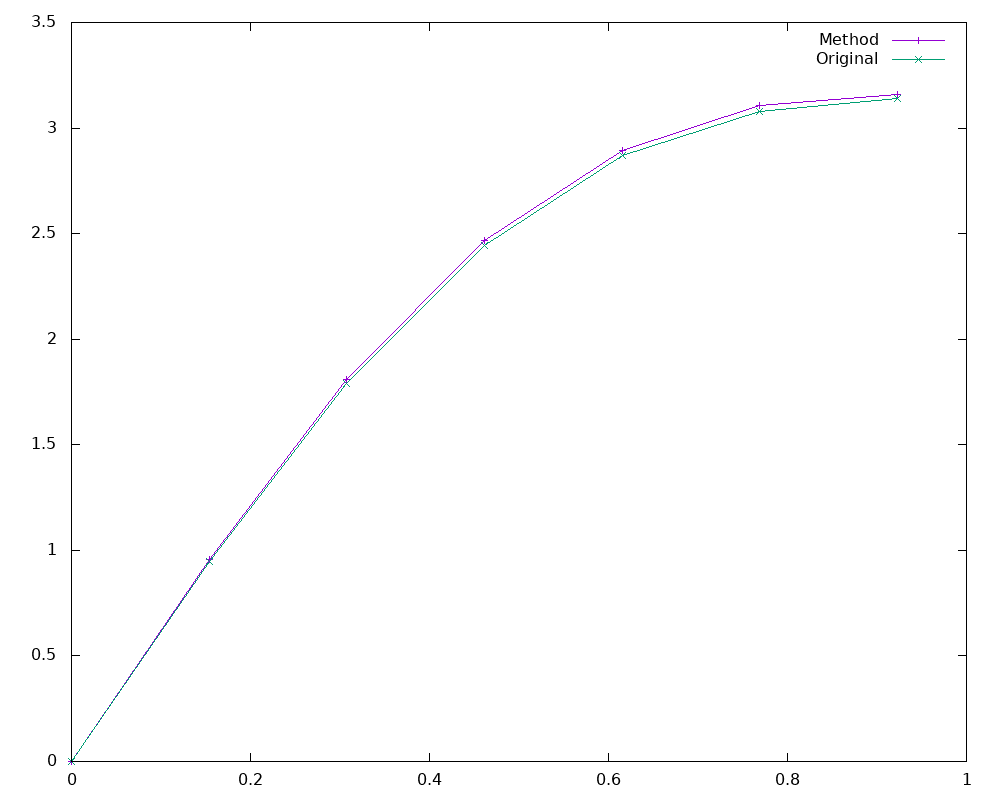
\includegraphics[width=12cm, height=8cm]{fourier_yn.png}

		      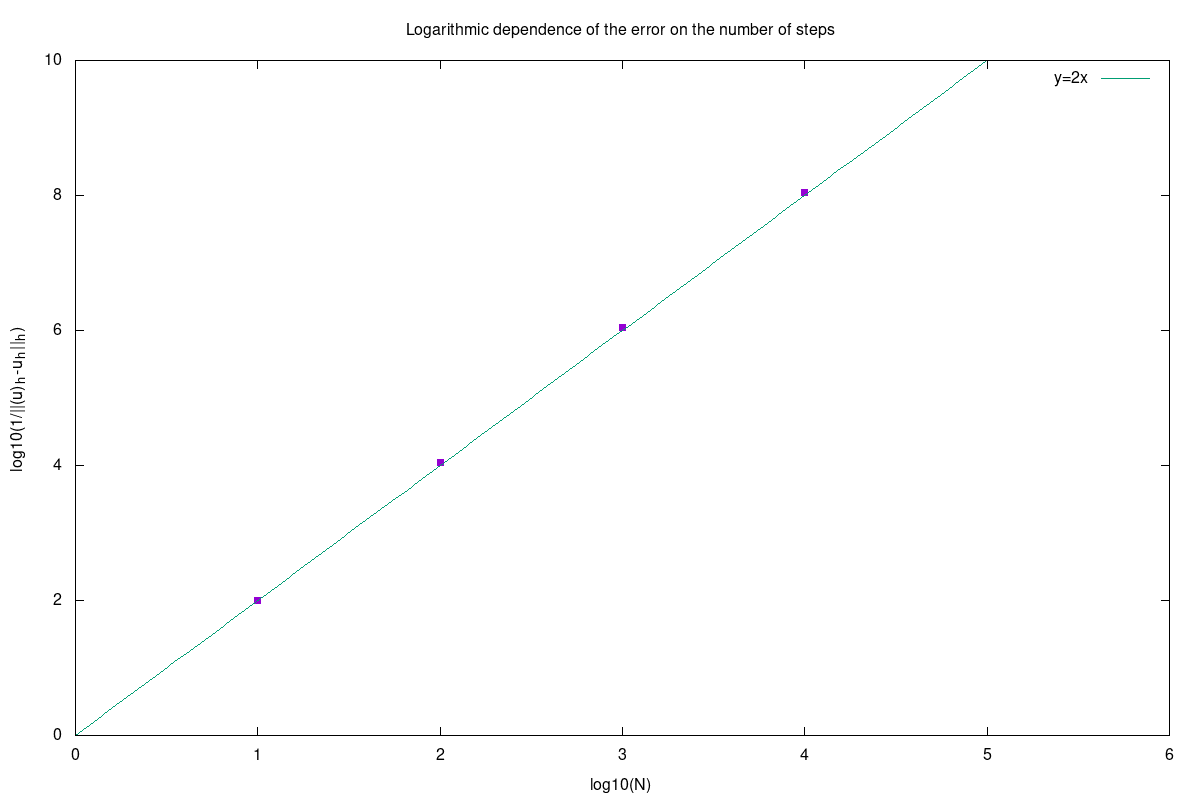
\includegraphics[width=12cm, height=8cm]{fourier_scale.png}

		      \begin{tabular}{c c}
			      $N$   & $\Vert(y)_h-y_h\Vert_h$ \\
			      10    & 1.004384e-02            \\
			      100   & 9.120604e-05            \\
			      1000  & 9.038345e-07            \\
			      10000 & 9.030208e-09            \\
		      \end{tabular}
	      \end{center}

	      \newpage

	      Метод прогонки показал:
	      \begin{center}
		      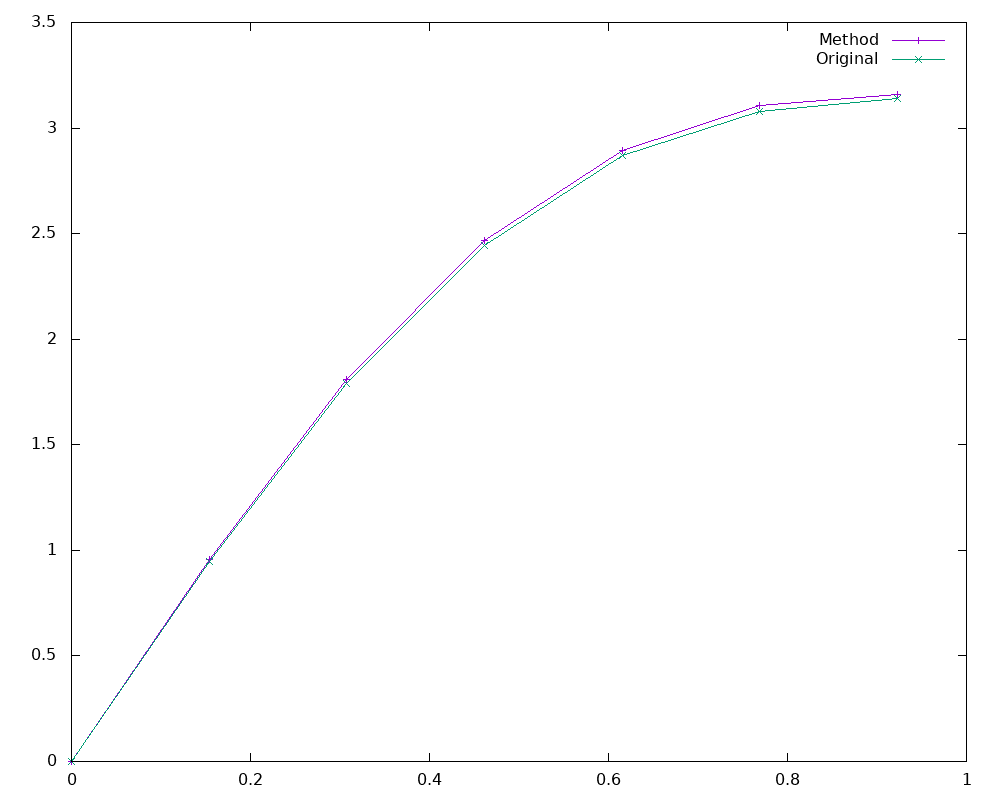
\includegraphics[width=12cm, height=8cm]{tridiag_yn.png}

		      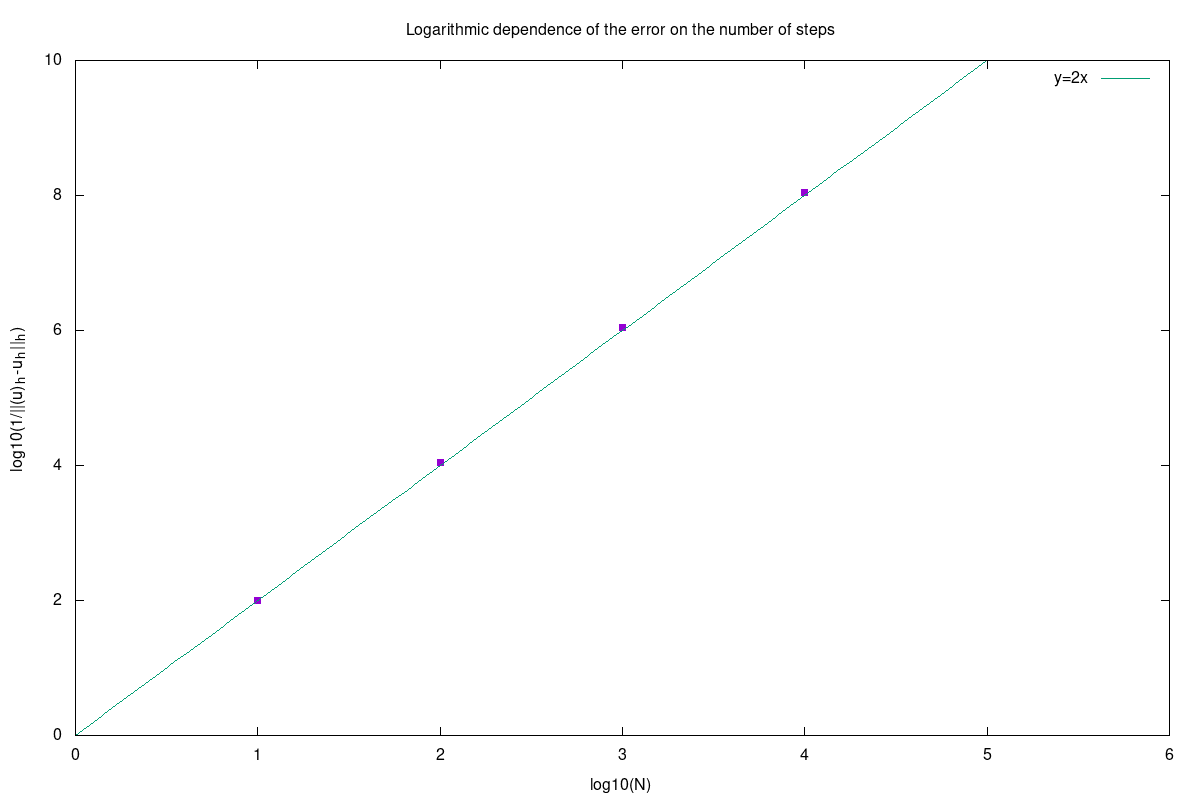
\includegraphics[width=12cm, height=8cm]{tridiag_scale.png}

		      \begin{tabular}{c c}
			      $N$   & $\Vert(y)_h-y_h\Vert_h$ \\
			      10    & 1.004384e-02            \\
			      100   & 9.120604e-05            \\
			      1000  & 9.038359e-07            \\
			      10000 & 9.092472e-09            \\
		      \end{tabular}
	      \end{center}

\end{enumerate}
\end{document}
